% $HeadURL$

\subsection{Glyph: \glyph{Perturbing agent}}
\label{sec:perturbing agent}

Biochemical networks can be affected by external influences.
Those influences can be the effect of well-defined physical perturbing agents, such as a light pulse or a change in temperature; they can also be more complex and not well-defined phenomena, for instance the outcome of a biological process, an experimental setup, or a mutation.
For these situations, \PD provides the \glyph{perturbing agent} glyph. It is an EPN, and represents the amount of perturbing agent applied to a process.

\begin{glyphDescription}

\glyphSboTerm
SBO:0000405 ! perturbing agent

\add{
\glyphIncoming
None.
}

\add{
\glyphOutgoing
One or more \glyph{modulation arcs} (\sect{modulations}) or \glyph{logic arcs} (\sect{logicArc}), zero or more \glyph{equivalence arcs} (\sect{equivalenceArc}).
}

\glyphContainer
A \glyph{perturbing agent} is represented by a by a modified hexagonal shape having two opposite concave faces, as shown in \fig{perturbing_agent}.

\glyphLabel
A \glyph{perturbing agent} is identified by a label that is \corr{an unbordered box containing}{} a string of characters \corr{.
The characters}{that} may be distributed on several lines to improve readability.
The centre of the label must be placed on the centre of the \corr{shape}{container}.
The label may extend outside of the \corr{shape}{container}.

\glyphAux
A \glyph{perturbing agent} can carry one or more \glyph{units of information} (\sect{unitInfo}).
% These can characterise <EXAMPLES>.
Particular \glyph{units of information} are available for describing the material type (\sect{material-types-cv}) and the conceptual type (\sect{conceptual-types-cv}) of a \glyph{perturbing agent}, as well as its physical characteristic (see \sect{physical-characteristics-cv}).

A \glyph{perturbing agent} can also carry a \glyph{simple clone marker} (see \sect{cloneMarker}).

\end{glyphDescription}

\begin{figure}[H]
  \centering
  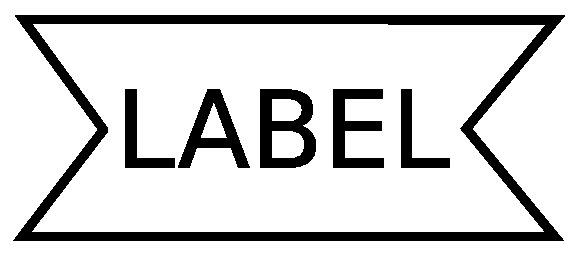
\includegraphics{images/perturbing_agent}
  \caption{The \PD glyph for \glyph{perturbing agent}.}
  \label{fig:perturbing_agent}
\end{figure}

% The following is for [X]Emacs users.  Please leave in place.
% Local Variables:
% TeX-master: "../sbgn_PD-level1"
% End:

